\addsection{Heroes}{\images/sorcery.png}
\hypertarget{Heroes}{Players} always control a main hero and may additionally also recruit a secondary hero.
A “player’s hero” may refer to either of them.
Heroes are used to perform movement actions on the game board and to start combats against enemies in order to reach a scenario victory condition.

\subsection*{Main hero}
The main hero is represented by its chosen model and hero card.
Each faction’s main hero has 3 movement points.
Only the main hero can use its own deck of cards.\par
Each main hero starts the game at level 1 and can advance up to level 7 by gaining experience.
Experience is gained from \hyperlink{Combatexperience}{winning combat}, visiting certain \hyperlink{All}{locations} and the \hyperlink{Resources}{treasure die} \includesvg[height=10px]{\svgs/trasuredie.svg}.
Gaining 1 experience is represented by the symbol \includesvg[height=10px]{\svgs/exp.svg}.

\subsection*{\hypertarget{Secondary}{Secondary heroes}}
If you control a town or a settlement, a secondary hero can be hired by flipping your population token and paying 10 gold.
\textbf{Note}: Units cannot be \hyperlink{Units}{recruited or reinforced} during that use of the population token.\par
Your secondary hero uses the remaining hero model of your faction.
You may wish to mark this model with a token such as a faction cube to differentiate it from the main hero.
After hiring a secondary hero, place the model in a town or settlement you control.
You can only have one secondary hero at a time.\par
Secondary heroes have 2 movement points.
When you gain a secondary hero, take an additional set of 2 movement tokens to represent their MP.
They do not have their own hero card, cannot gain experience, and cannot use your cards from your deck for any reason.
If a secondary hero gains any cards, place them into your hand as normal.
Secondary heroes are considered to have the same level as the main hero for the purposes of resolving \hyperlink{Quick}{quick combat} against neutral enemies.\par
If your secondary hero is attacked by an enemy hero, you can choose to have your hero be \hyperlink{Endcombat}{instantly defeated instead of fighting a combat}.
When a secondary hero is defeated, remove them from the game.
They can be recruited again with another use of the population token.\par

\clearpage

\subsection*{\hypertarget{Herocard}{Hero Card Anatomy}}
\bigbreak
\begin{figure}[h]
  \begin{minipage}[t]{0.5\textwidth}
    \vspace{0pt}
    \begin{enumerate}[itemsep=5pt]
      \item \textbf{Name} – The hero’s name.
        Used for identification.
        Has no gameplay effect.
      \item \textbf{Class} – The hero’s class.
        Has no gameplay effect.
      \item \textbf{Type} – The hero’s type (might \includesvg[height=10px]{\svgs/might.svg} or magic \includesvg[height=10px]{\svgs/magic.svg}).
        Determines the amount of magic arrow spells in your starting deck (1 or 2 respectively).
      \item \textbf{Faction color} – Reminder for the color of the faction’s cubes and miniatures.
      \item \textbf{Attack} – Number of attack cards in your starting deck.
      \item \textbf{Defense} – Number of defense cards in your starting deck.
      \item \textbf{Power} – Number of power cards in your starting deck.
      \item \textbf{Knowledge} – Number of knowledge cards in your starting deck.
      \item \textbf{Starting Ability} – Reminder for the unique ability card the hero starts with.
      \item \textbf{Hero Specialty} – Reminder for the specialty cards the hero adds to their deck at the start of the game and after specific level ups.
        Each hero has three specialty cards.
      \item \textbf{Level tracker} – Whenever a main hero gains 1 or more experience \includesvg[height=10px]{\svgs/exp.svg} move the cube that number of steps on this track.
        When the cube reaches the next slot on the upper row, the hero gains a level.
    \end{enumerate}
  \end{minipage}\hfill
  \begin{minipage}[t]{0.48\textwidth}
    \centering
    \vspace{0pt}
    \begin{scriptsize}
      \begin{tikzpicture}
        \draw (0, 0) node[inner sep=0] {\makebox[\textwidth][c]{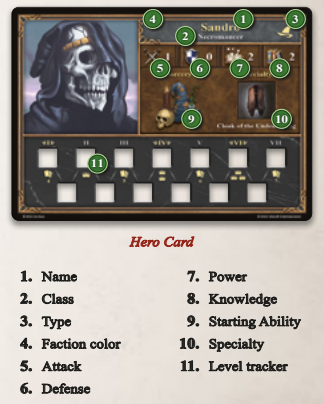
\includegraphics[width=\linewidth]{\images/herocard.png}}};
        \draw (2.3, 2.5) node {\encircle{\phantom{.}1\phantom{.}}};
        \draw (0.8, 1.9) node {\encircle{\phantom{.}2\phantom{.}}};
        \draw (3.5, 2.5) node {\encircle{\phantom{.}3\phantom{.}}};
        \draw (-0.1, 2.5) node {\encircle{\phantom{.}4\phantom{.}}};
        \draw (0, 1.25) node {\encircle{\phantom{.}5\phantom{.}}};
        \draw (1.1, 1.25) node {\encircle{\phantom{.}6\phantom{.}}};
        \draw (2, 1.25) node {\encircle{\phantom{.}7\phantom{.}}};
        \draw (3.25, 1.25) node {\encircle{\phantom{.}8\phantom{.}}};
        \draw (1, -0.2) node {\encircle{\phantom{.}9\phantom{.}}};
        \draw (3, -0.2) node {\encircle{10}};
        \draw (-1.7, -1.4) node {\encircle{11}};
      \end{tikzpicture}
    \end{scriptsize}
    \break
    \footnotesize{\textbf{\textit{\textcolor{darkcandyapplered}{Hero Card}}}}
    \scriptsize
    \begin{multicols}{2}
      \begin{itemize}
        \item[\textbf{1.}] \textbf{Name}
        \item[\textbf{2.}] \textbf{Class}
        \item[\textbf{3.}] \textbf{Type}
        \item[\textbf{4.}] \textbf{Faction color}
        \item[\textbf{5.}] \textbf{Attack}
        \item[\textbf{6.}] \textbf{Defense}
        \item[\textbf{7.}] \textbf{Power}
        \item[\textbf{8.}] \textbf{Knowledge}
        \item[\textbf{9.}] \textbf{Starting Ability}
        \item[\textbf{10.}] \textbf{Specialty}
        \item[\textbf{11.}] \textbf{Level tracker}
        \item[\textbf{\phantom{.}}] \phantom{.}
      \end{itemize}
    \end{multicols}
  \end{minipage}
\end{figure}

\clearpage

\subsection*{\hypertarget{Level}{Level effects}}
Main Heroes always start each scenario at Level 1 and may Level up by gaining Experience \includesvg[height=10px]{\svgs/exp.svg}.
The most common sources of gaining experience are the \hyperlink{Resources}{treasure die} and \hyperlink{Combatexperience}{combat}.
Each new level up requires \textbf{2 Experience}.
When a main hero reaches a new level, resolve the effects of the level up immediately.
If a main hero gains multiple levels at the same time, resolve the effects in ascending level order.
Gaining experience at level 7 has no effect.\par
The level tracker on your hero card shows the following information:
\begin{itemize}
\item Your main hero’s current level and amount of experience gained, shown by the cube's position.
\item Your current hand limit \includesvg[height=10px]{\svgs/hand.svg}.
\item The number of \hyperlink{Ability}{expert effects} \includesvg[height=10px]{\svgs/expert.svg} you may use during a round.
\item At which levels your main hero must \hyperlink{Playerdecks}{Search} for a new \hyperlink{Ability}{Ability card} or gain a \hyperlink{Specialty}{specialty card}.
Level numbers written in gold on the level tracker (\includesvg[height=10px]{\svgs/level1.svg}, \includesvg[height=10px]{\svgs/level4.svg} and \includesvg[height=10px]{\svgs/level6.svg}) give you a Specialty card, while silver levels (2, 3, 5, 7) give you an Ability card.
\end{itemize}
List of all effects:
\begin{itemize}
\item \textbf{Level 1} – Your hand limit is 4.
Add your first specialty card to your deck.
\item \textbf{Level 2} – Search (2) the ability deck.
You may play 1 card for their expert effect per round.
\item \textbf{Level 3} – Your hand limit is 5.
Search (2) the ability deck.
\item \textbf{Level 4} – Gain your second specialty card.
You may play 2 cards for their expert effect per round.
\item \textbf{Level 5} – Your hand limit is 6.
Search (2) the ability deck.
\item \textbf{Level 6} – Gain your third specialty card.
You may play 3 cards for their expert effect per round.
\item \textbf{Level 7} – Your hand limit is 7.
Search (2) the ability deck.
\end{itemize}
